\section{Аппроксимация функций}
\subsection{Аппроксимация в пространствах $L_p$}
Для наших целей понадобится приближать наши функции другими, более понятными.

\begin{definition}
    Функция $f : \R^{n} \rightarrow \R$ называется ступенчатой, если она является линейной комбинацией индикаторов ячеек. Ячейкой называют $P = \sqcap_{i=1}^n[a_i, b_i)$.
\end{definition}

Теперь докажем, что такие функции приближают по норме $L_p$.

\begin{theorem}
    Пусть множество $E \subseteq \R^n$ измеримо, $f \in L_p(E), $ где $p \in [1, +\infty)$.
    Тогда верно следующее:
    $$\forall \varepsilon > 0 \ \exists \ \text{ступенчатая функция } h_{\varepsilon} : ||f - h_{\varepsilon}||_{L_p(E)} < \varepsilon.$$
\end{theorem}

\underline{Идея доказательства:} как обычно мы доказываем это сначала для простых функций, а позже для всех, сводя к уже доказанному с помощью приближений.

\begin{proof} Разобьем доказательство на шаги:

\textit{Шаг 1.} Пусть $f = \chi_{G},$ где множество $G$ имеет конечную меру. Тогда из определения верхней меры следует:
    $$\forall \varepsilon > 0 \ \exists \{P_{k}\}_{k = 1}^{\infty} : \ \LL^n(G) + \varepsilon \geq \sum_{k  =1}^{\infty}\LL(P_k).$$
    Теперь из сходимости ряда мер ячеек следует, что можно взять такой большой номер $N:$
    $$\sum_{k = N + 1}^{\infty} \LL^n(P_k) < \varepsilon.$$
    По теореме о дизъюнктном представлении в полукольце существует набор непересекающихся $\{Q_l\}_{l = 1}^{m}: \ P_1 \cup \ldots \cup P_N = \bigsqcup_{l = 1}^mQ_l.$ Обозначим за $A = \bigcup_{i = 1}^{\infty} P_k, \text{ а также } B = P_1 \cup \ldots \cup P_N.$ Тогда
    $$h = \chi_B= \sum_{l = 1}^{m}\chi_{Q_l}.$$
    Возьмем в качестве приближающей ступенчатой функции $h$ Осталось доказать, что она приближает с точностью до $\varepsilon$ по норме.
    $$||f - h||_{L_p} = \left( \int_{\R^n} |\chi_G(x) - \chi_B(x)|^p dx\right)^{\frac{1}{p}} \leq$$
    $$\leq \left( \int_{\R^n} |\chi_G(x) - \chi_A(x)|^p dx\right)^{\frac{1}{p}} + \left( \int_{\R^n} |\chi_A(x) - \chi_B(x)|^p dx\right)^{\frac{1}{p}} = $$
    $$= \left( \LL^n(A \setminus G)\right)^{\frac{1}{p}} + \left( \LL^n(A \setminus B) \right)^{\frac{1}{p}} \leq 2\varepsilon^{\frac{1}{p}}.$$
\textit{Шаг 2.} Если $f$ -- простая, то есть линейная комбинация индикаторов множеств конечной меры, явно сводится к пункту $1$ с помощью неравенства треугольника.\\   
\textit{Шаг 3.} $f \in L_p(E)$ произвольная, тогда из определения интеграла Лебега можно ее приблизить простой с точностью до $\varepsilon / 2, $а простые мы уже умеем приближать ступенчатыми с точностью до $\varepsilon / 2.$ Осталось применить неравенство треугольника и требуемое будет доказано.
\end{proof}

Теперь мы можем показать непрерывность интеграла Лебега по сдвигу.
\begin{theorem}[Непрерывность по сдвигу]
    Пусть $f \in L_p(\R^n), $ где $p \in [1, +\infty).$ Тогда верно следующее:
    $$||f(x) - f(x - h)||_{L_p} \rightarrow 0, h \rightarrow 0$$
\end{theorem}

\underline{Идея доказательства:} Обозначим за $f_h(x) = (x - h),$ заметим, что в силу неравенства треугольника:
$$||f - f_h|| \leq ||f - g|| + ||g - g_h|| + ||f_h - g_h|| \ \forall g \in L_p(\R^n)$$
Ясно, что можно $g$ можно подобрать, чтобы 1 и 3 слагаемые были маленькими, проблема лишь в том, чтобы уменьшить второе слагаемое.

\begin{proof}
    Заметим, что для любой функции $g \in L_p(\R^n):$
    $$||f_h - g_h||_p = \left( \int_{\R^n}|f(x - h) - g(x - h)| dx\right)^{\frac{1}{p}} = \{\text{выполним замену переменной } t = x - h\}=$$
    $$= \left ( \int_{\R^n} |f(t) - g(t)| dt\right)^{\frac{1}{p}} = ||f - g||_p$$
    Тогда в качестве $g$ возьмем ступенчатую функцию, которая приближает $f.$ Осталось теперь доказать, что $g$ можно приблизить $g_h.$ Из теоремы о дизъюнктном представлении следует, что $g$ можно представить в виде:
    $$g(x) = \sum_{k = 1}^{n}a_k \chi_{Q_k}(x), \ Q_k -\text{ячейка}$$
    $$||g - g_h||_p \leq \sum_{k = 1}^{n} |a_k| \cdot ||\chi_{Q_k} - \chi_{Q_k + h}||$$
    Что стремится к нулю при $h \longrightarrow 0.$
\end{proof}

\subsection{Свёртка функций}

\begin{lemma}
    Пусть $f: \R^n \rightarrow \R$ измеримая функция, тогда отображения
    $$(x, y) \mapsto f(x - y)$$
    $$(x, y) \mapsto f(x + y)$$
    измеримы как отображения $\R^{2n} \to \R$.
\end{lemma}

\begin{proof}
    Докажем первое утверждение, второе доказывается аналогично. Обозначим за $E_c = \{x | \ f(x) > c\},$ оно является измеримым из условия леммы. Теперь рассмотрим следующее линейное отображение:
    $$T: (x, y) \longrightarrow (x - y, y).$$
    Оно обратимо, так как определено обратное отображение $T^{-1}((x, y)) = (x + y, y).$ Осталось лишь заметить, что верно:
    $$\{(x, y) | x - y \in E_c\} = T^{-1}(E_C \times \R^n) = \{(x, y) | \ f(x - y) > c\} .$$
    Отсюда следует требуемое.
\end{proof}

Теперь мы готовы к определению свертки функций и к доказательству корректности этого определения.

\begin{theoremdefinition}
    Пусть $f, g \in L_1(\R^n).$ Тогда
    \begin{enumerate}
        \item Для $\LL-$почти всех $x \in \R^n$ корректно определена функция (будет называть ее сверткой) $f*g(x) := \int_{\R^n}f(x - y)g(y) dy.$
        \item $f* g$ измерима в широком смысле.
        \item $f * g \in L_1(\R^n)$
        \item $||f * g||_{L_1} \leq ||f||_{L_1} \cdot ||g||_{L_1}$
    \end{enumerate}
\end{theoremdefinition}

\begin{proof}
    Рассмотрим следующую функцию:
    $$H(x, y) = |f(x - y)| \cdot |g(y)|.$$
    Ясно, что это неотрицательная, измеримая функция, тогда по теореме Тонелли:
    $$\iint_{\R^{2n}}H(x, y) dx dy = \int_{\R^n}\left( \int_{\R^n} H(x, y) dy\right) dx = \int_{\R^n}\left( \int_{\R^n} H(x, y) dx\right) dy.$$
    Подробнее остановимся на втором интеграле, внутренний интеграл преобразуется так(последнее равенсвто получается заменой переменной $t = x-y$):
    $$\int_{\R^n} H(x, y) dx = \int_{\R^n} |f(x - y)| \cdot |g(y)| dx = |g(y)| \int_{\R^n}|f(x - y)|dx = |g(y)| \cdot ||f||_{L_1}$$
    Тогда весь интеграл:
    $$ \int_{\R^n}\left( \int_{\R^n} H(x, y) dx\right) dy = ||f||_{L_1} \cdot  \int_{\R^n} |g(y) dy = ||f||_{L_1} \cdot ||g||_{L_1} < + \infty$$
    Получили, что $H \in L_1(\R^{2n})$. А если теперь применим теорему Фубини для $F(x, y) = f(x - y) g(y),$ так как выше мы показали, что $F(x, y) \in L_1(\R^{2n}).$ Тогда пункты $1, 2$ из нее сразу следуют. Покажем оставшиеся:
    $$\int_{\R^n}|f*g|(x) dx \leq \int_{\R^n}\left( \int_{\R^n} |f(x - y)| \cdot |g(y)| dy \right) dx = ||f||_{L_1} \cdot ||g||_{L_1}$$
\end{proof}

Сформулируем еще одну теорему

\begin{theorem}
    Пусть $p \in [1, +\infty), \ f \in L_p(\R^n), \ g \in L_{p'}(\R^n), $ где $\frac{1}{p} + \frac{1}{p'} = 1.$ Тогда:
    \begin{enumerate}
        \item $f * g(x)$ корректно определена для всех $x \in \R^n.$
        \item $f * g(x)$ равномерно непрерывна на $R^n.$
    \end{enumerate}
\end{theorem}

\begin{proof}
Докажем последовательно
    \begin{enumerate}
        \item По неравенству Гельдера получаем:
        $$|f * g(x)| \leq \int_{R^n}|f(x - y)| \cdot |g(y)| dy \leq ||f||_{L_p} \cdot ||g||_{L_{p
        '}} < + \infty$$
        \item Обозначим за $(f * g)_h(x) = f * g(x - h), f_h(x) = f(x -h).$ Верно равенство:
        $$(f * g)_h(x) - f * g(x) = \int_{R^n} f(x - y -h) g(y)dy - f*g(x) = f_h * g(x) - f*g(x)$$
        Теперь оценим отклонение свертки при сдвиге:
        $$|(f * g)_h(x) - f * g(x)| = |f_h * g(x) - f*g(x)| \leq ||f_h - f| * g(x)| \leq ||f-f_h||_{L_p} \cdot ||g ||_{L_p'}$$
        Теперь по уже доказанному утверждению,  получаем, что правая часть стремится к $0$ и при этом оценка не зависит от $x.$ Таким образом, требуемое доказано.
        \item Осталось рассмотреть случаи, когда одно из $p, p'$ равно $+\infty.$ А именно рассмотрим случай, когда $p = \infty, p' = 1.$ Для этого случая достаточно лишь заметить, что совершенно аналогично доказывается неравенство:
        $$|f * g(x)| \leq ||f||_{L_1} \cdot ||g||_{L_{\infty}}$$
    \end{enumerate}
\end{proof}

\subsection{Аппроксимативная единица}
\begin{definition}
    Пусть $f: \R^n \rightarrow \R$. Носителем функции будем называть множество $\supp \ f = cl{\{x \in \R^n : f(x) \neq 0 \}}$ (замыкание множества точек где функция не нулевая)
\end{definition}

\begin{definition}
    Семейство функций $\{\omega_t\}_{t \in (0, +\infty)}$ называется аппроксимативной единицей, если $\forall t > 0$ выполнено следующее:
    \begin{enumerate}
        \item $\omega_t(x) \ge 0 \ \forall x \in \R^n$.
        \item $\int\limits_{\R^n} \omega_t(x) dx = 1$.
        \item Выполнено фокусирующее свойство: \[\forall \delta > 0  \ \exists \lim\limits_{t \ra +0} \int\limits_{\R^n \setminus B_\delta(0)} \omega_{t}(x)dx = 0.\]
    \end{enumerate}
\end{definition}
Интуитивно ожидается, что графики функций \(\omega_t(x)\) при \(t \to 0\) образуют семейство всё более узких и высоких «колоколов», концентрирующихся в окрестности нуля и сохраняющих единичную площадь.
\begin{center}
    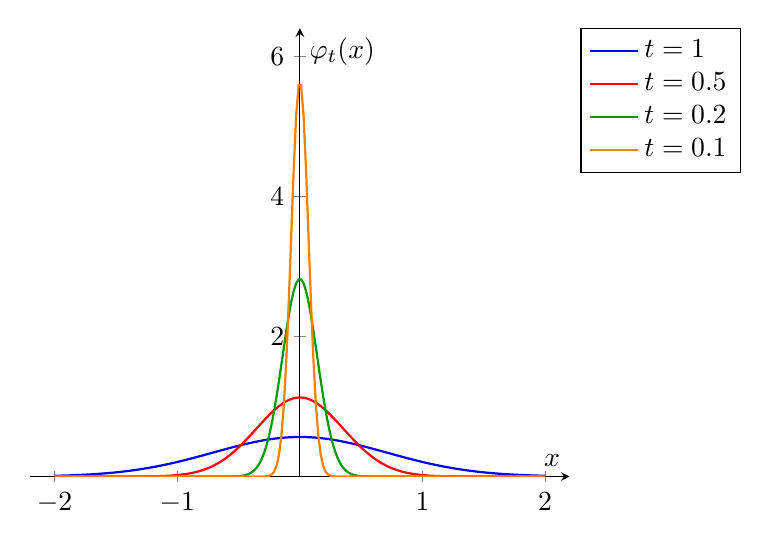
\begin{tikzpicture}
  \begin{axis}[
      axis lines=middle,
      xlabel={$x$},
      ylabel={$\varphi_t(x)$},
      xmin=-2.2, xmax=2.2,
      ymin=0, ymax=6.4,
      samples=200,
      domain=-2:2,
      legend style={at={(1.02,1)}, anchor=north west},
      legend cell align=left,
      every axis plot/.append style={thick},
    ]
    % t = 1
    \addplot[blue] {1/(1*sqrt(pi))*exp(-(x/1)^2)};
    \addlegendentry{$t=1$}

    % t = 0.5
    \addplot[red] {1/(0.5*sqrt(pi))*exp(-(x/0.5)^2)};
    \addlegendentry{$t=0.5$}

    % t = 0.2
    \addplot[green!60!black] {1/(0.2*sqrt(pi))*exp(-(x/0.2)^2)};
    \addlegendentry{$t=0.2$}

    % t = 0.1
    \addplot[orange] {1/(0.1*sqrt(pi))*exp(-(x/0.1)^2)};
    \addlegendentry{$t=0.1$}
  \end{axis}
\end{tikzpicture}
\end{center}




\begin{note}
	В нашем курсе мы предъявляем дополнительные требования к аппроксимативной единице:
	\begin{itemize}
		\item $\forall t \in (0, +\infty) \hookrightarrow w_t$ -- непрерывны и имеют компактный носитель
	\end{itemize}
    \begin{definition}
        Нижний индекс $0$ у пространства $C_0^n(\Omega)$ означает, что рассматриваются функции из $C^n(\Omega)$, имеющие компактный носитель в области $\Omega$. 
    \end{definition}
    
	Тогда справедливо следующее утверждение:
	\begin{theorem}
		Если $f \in L_1^{loc}(\R^n)$ и $w_t$ -- аппроксимативная единица (произвольная в смысле нашего определения), то их свёртка является корректно определённой непрерывной функцией.
	\end{theorem}
	\begin{proof}
		Если $f \in L_1(\R^n)$, то утверждение является частным случаем теоремы о свёртке функций из $L_p$ и $L_{p'}$: и действительно, $f \in L_1(\R^n)$, а всякая непрерывная функция с компактным носителем ограничена и, как следствие, лежит в $L_{\infty}(\R^n)$.
		Тогда $f * w_t$ -- корректно всюду определённая равномерно непрерывная функция. \\
		Пусть теперь $f \in L_1^{loc}(\R^n)$.
		Пусть $\supp w_t \subset B(r)$, где $B(r)$ -- некоторый замкнутый шар радиуса $r$ с центром в 0.
		Положим $H(x) = |f(x - y)||w_t(y)|$.
		Заметим, что на всяком шаре $B(R) \subset \R^{m}$ функция $H$ интегрируема:
		\begin{multline*}
			\int_{B(R)} H(x)dx = \int_{B(R)} \biggr(\int_{\R^n}|f(x - y)||w_t(y)|dy\biggr)dx = \\ = \int_{B(r)} |g(y)| \biggr(\int_{B(R)} |f(x - y)|dx \biggr) dy \leq \int_{B(r)} |w_t(y)|dy \int_{B(R + r)} |f(z)|dz < +\infty.
		\end{multline*}
		Таким образом $H(x)$ конечна почти всюду на всяком замкнутом шаре, а следовательно почти всюду конечна и на всём пространстве и свёртка определена корректно. \\
		Заметим, что $f * w_t$ и $f\chi_{B(R + r)} * w_t$ совпадают в шаре $B(R)$, поскольку если $x \in B(R + r), y \in B(r)$ то $\|x\| \leq R$ и $\|y\| \leq r$, то $\|x - y\| \leq R + r$ и следовательно
		\[
		f * w_t(x) = \int_{B(r)} f(x - y)w_t(y)dy = \int_{B(r)} f(x - y)\chi_{B(R + r)}(x - y)w_t(y)dy = f\chi_{B(R + r)} * w_t.
		\]
		Поскольку на непрерывность функции $f * w_t$ в точке влияет её поведение только в некоторой окрестности, то мы можем рассмотреть $f\chi_{B(R + r)}$ -- уже интегрируемую функцию -- и её свёртка с $w_t$ будет непрерывной, а следовательно, в силу совпадения свёрток в $B(R)$, то и для всякой точки оттуда $f * w_t$ -- непрерывна.
		Поскольку $R$ было выбрано произвольно, то $f * w_t$ непрерывна на всём пространстве.
	\end{proof}
\end{note}

\begin{example}[Соболевская аппроксимативная единица]
    Соболевской <<шапкой>> будем называть функцию
    \[
        \psi(x) = \begin{cases}
                      \exp\biggr({-\dfrac{1}{1 - \|x\|^2}}\biggr), & \|x\| < 1 \\
                      0, & \text{ иначе.}
        \end{cases}
    \]
    Функция $\psi \in C^{\infty}(\R^n)$ и её носитель -- замкнутый единичный шар. \\
    Обозначим $\int_{\R^n} \psi(x)dx = C \neq 0$ ~---~ некоторая константа. \\
    Обозначим за $\omega = \psi/C$.
    Тогда $\omega$ -- неотрицательная, бесконечно гладкая функция с компактным носителем и единичным интегралом по всему пространству. \\
    Положим по определению \[
\omega_\varepsilon(x) := \frac{1}{\varepsilon^n} \, \omega\left( \frac{x}{\varepsilon} \right), \varepsilon > 0
\]
    Семейство функций $\{\omega_\epsilon\}_{\epsilon \in (0, +\infty)}$ является аппроксимативной единицей.
\end{example}
\begin{definition}
        Пусть $f \in L_p(\R^n)$.
    Усреднением $f$ по Соболеву будем называть функцию $f_\epsilon = f * \omega_\epsilon$.
    По предыдущей теореме, $f_\epsilon$ -- всюду корректно определённая непрерывная функция.
\end{definition}

\begin{note}
    Далее в курсе будет доказано, что $f_\epsilon \in C^{\infty}(\R^n)$.
\end{note}

Докажем техническую лемму, которая будет использована в дальнейшем доказательстве.
    \begin{lemma}
        Пусть $\{w_t\}_{t \in (0, +\infty)}$ -- аппроксимативная единица и $g: \R^n \to \R$ -- измеримая ограниченная функция такая, что $g(x) \ra 0, x \ra 0$.
        Тогда верно следующее:
        \[
            \int_{\R^n} g(x)w_t(x)dx \ra 0, t \ra +0.
        \]
    \end{lemma}
    \begin{proof}
        Для всякого $\delta > 0$ выполняется следующее:
        \[
            \int_{\R^n} gw_t dx = \int_{\|x\| \geq \delta} gw_t dx + \int_{\|x\| < \delta} gw_t dx = I_1(\delta) + I_2(\delta).
        \]
        Поскольку $g$ -- ограниченная функция, существует $M > 0$ такое, что $|g| \leq M$.
        Поэтому
        \[
            |I_1(\delta)| \leq M \int_{\|x\| \geq \delta} w_t dx.
        \]
        Из определения аппроксимативной единицы следует
        \[
            M \int_{\|x\| \geq \delta} w_t dx \ra 0, t \ra  +0.
        \]
        Тогда и $|I_1(\delta)| \ra 0, t \ra +0$.
        Теперь оценим второй интеграл:
        \[
            |I_2(\delta)| = \biggr|\int_{\|x\| < \delta}g w_t dx\biggr| \leq \int_{\|x\| < \delta} |g|w_t dx \leq \sup\limits_{\|x\| < \delta} g \int_{\|x\| < \delta} w_t dx \leq \sup\limits_{\|x\| < \delta} g.
        \]
        (где последний переход сделан из тех соображений, что $\int_{\R^n} w_t dx = 1$)
        Поскольку $g$ -- непрерывна в нуле, то $I_2(\delta)$ может быть сделан сколь угодно малым и, следовательно, утверждение леммы показано.
    \end{proof}

\begin{theorem}
    Пусть $p \in [1, +\infty)$ и $f \in L_p(\R^n)$. Тогда
    \[
        \forall \epsilon > 0  \ \exists h \in C^{\infty}_0(\R^n) \hookrightarrow \|f - h\|_p \leq \epsilon.
    \]
\end{theorem}
\begin{proof}
    Зафиксируем $\epsilon > 0$.
    Из свойств интеграла Лебега следует, что $\exists R > 0$ такое, что
    \[
        \biggr(\int_{\R^n \setminus B_R(0)} |f|^p dx\biggr)^{1/p} < \epsilon.
    \]
    Это в точности означает что для функции $g = \chi_{B_R(0)}f$ выполняется
    \[
        \|f - g\|_p \leq \epsilon.
    \]
    
    Пусть теперь $w_t$ -- соболевская аппроксимативная единица.
    Поскольку $g$ -- локально интегрируемая функция то $g * w_t$ определена корректно и, так как $w_t \in C_0^\infty(\R^n)$, то и $g * w_t \in C_0^\infty(\R^n)$.
    Заметим, что для доказательства теоремы достаточно показать что $\|g - g * w_t\|_p \ra 0, t \ra +0$.
    Распишем подробнее вид $|g - g * w_t|$:
    \begin{multline*}
        |g - g * w_t|(x) = \biggr| g(x) - \int_{\R^n} g(x - y)w_t(y)dy \biggr| = \biggr|\int_{\R^n} g(x)w_t(y)dy - \int_{\R^n} g(x - y)w_t(y)dy\biggr| = \\ = \biggr|\int_{\R^n} (g(x) - g(x - y))w_t\biggr| \leq \int_{\R^n} |g(x) - g(x - y)|w_t(y)dy.
    \end{multline*}
    В тоже время, мы можем расписать $|g(x) - g(x - y)|w_t$ как \[|g(x) - g(x - y)|w_t = (|g(x) - g(x - y)|w_t^{1/p}(x)) \cdot w_t^{1/p'}(x).\]
    и применить неравенство Гёльдера:
    \[
        \||g(x) - g(x - y)|w_t\|_1 \leq \||g(x) - g(x - y)|w_t^{1/p}\|_p \cdot \|w_t^{1/p'}\|_{p'} = \||g(x) - g(x - y)|w_t^{1/p}|\|_p.
    \]
    И тогда
    \[
        |g - g * w_t|(x) \leq \biggr( \int_{\R^n}|g(x) - g(x - y)|^p w_t(y)dy \biggr)^{1/p}.
    \]
    Возведём $|g - g * w_t|(x)$ в $p$-ую степень и проинтегрируем по всему пространству.
    В силу ранее полученной оценки мы получим:
    \[
        \int_{\R^n}|g - g * w_t|^p dx \leq \int_{\R^n} \int_{\R^n} |g(x) - g(x - y)|^p w_t dy dx = \int_{\R^n} w_t(y) \biggr(\int_{\R^n} |g(x) - g(x - y)|^{p} dx \biggr) dy.
    \]
    (где мы поменяли пределы интегрирования в силу теоремы Фубини).
    Обозначим за $s(y) = \int_{\R^n}|g(x) - g(x - y)|^p dx$.
    Из непрерывности по сдвигу для $p$-й нормы $s(y) \ra 0, y \ra 0$ -- а следовательно мы можем применить ранее доказанную лемму к $\int_{\R^n}w_t(y)s(y)dy$ и получить нужное утверждение:
    \[
        \|g - g * w_t\|_p \ra 0, t \ra +0.
    \]
    Значит $\forall \epsilon > 0 \exists t_{\epsilon}$ такое, что $\|g - g * w_{t_\epsilon}\|_p < \epsilon$.
    Таким образом $h = g * w_{t_\epsilon}$ -- искомое:
    \[
        \|f - h\|_p \leq \|f - g\|_p + \|g - h\|_p < 2\epsilon.
    \]
\end{proof}